\documentclass[11pt]{article}
\usepackage{graphicx}  % this is the up-to-date package for all figures
\usepackage{float}	% allows use of 'H' command
\usepackage{subcaption} % for sub-captions on side-by-side figures


% these are some custom control of the page size and margins
% \topmargin= 0.2in  % these 1st two may be needed for some computers
%\textheight=8.75in
\textwidth=6.5in
\oddsidemargin=0cm
\evensidemargin=0cm


% this is where the actual document itself (rather than control statements) begins:

\begin{document}

% Use relative calling to reference the images
\begin{figure}[H]
\centering
  \begin{subfigure}{.5\textwidth}
    \centering
      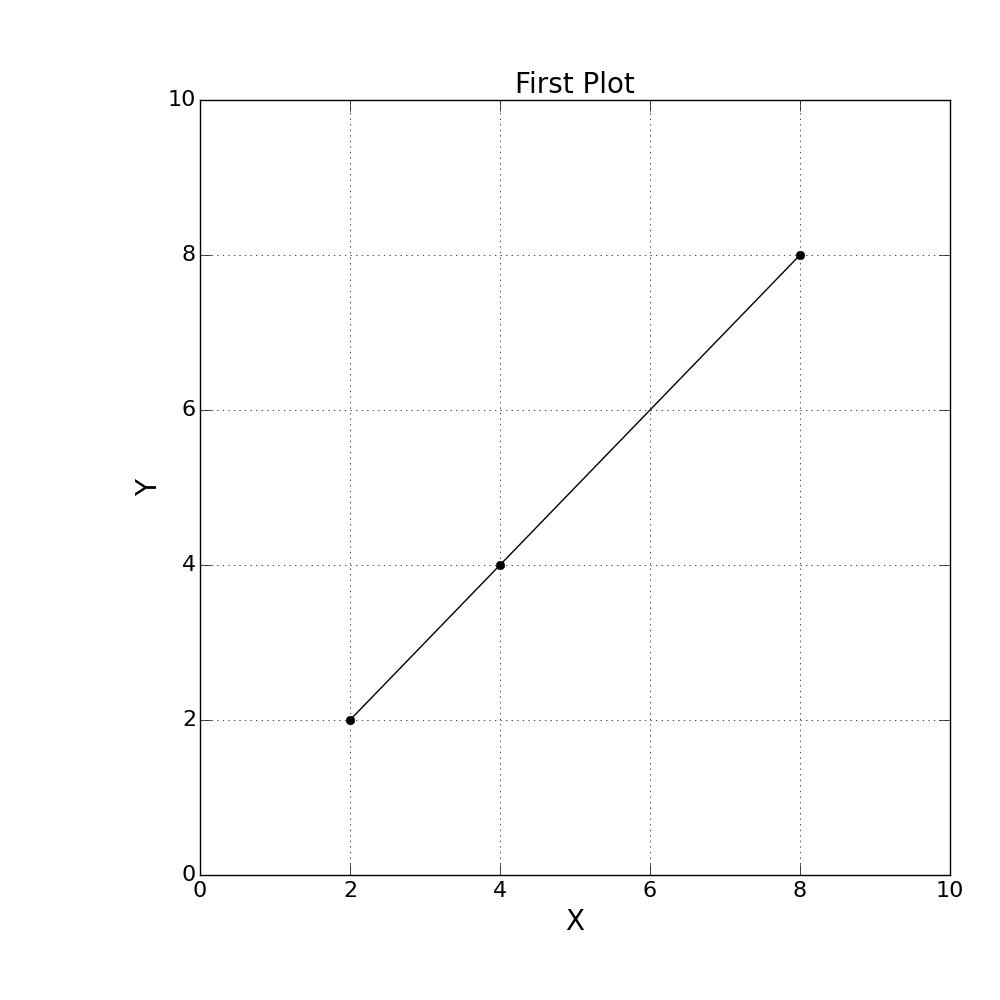
\includegraphics[width=1\linewidth]{../Python/LinePlot/lp.png}
      \caption{\it \small{foo}}
        \label{fig:na4}
  \end{subfigure}%
  % if this line were blank, the figures would stack vertically
  \begin{subfigure}{.5\textwidth}
    \centering
      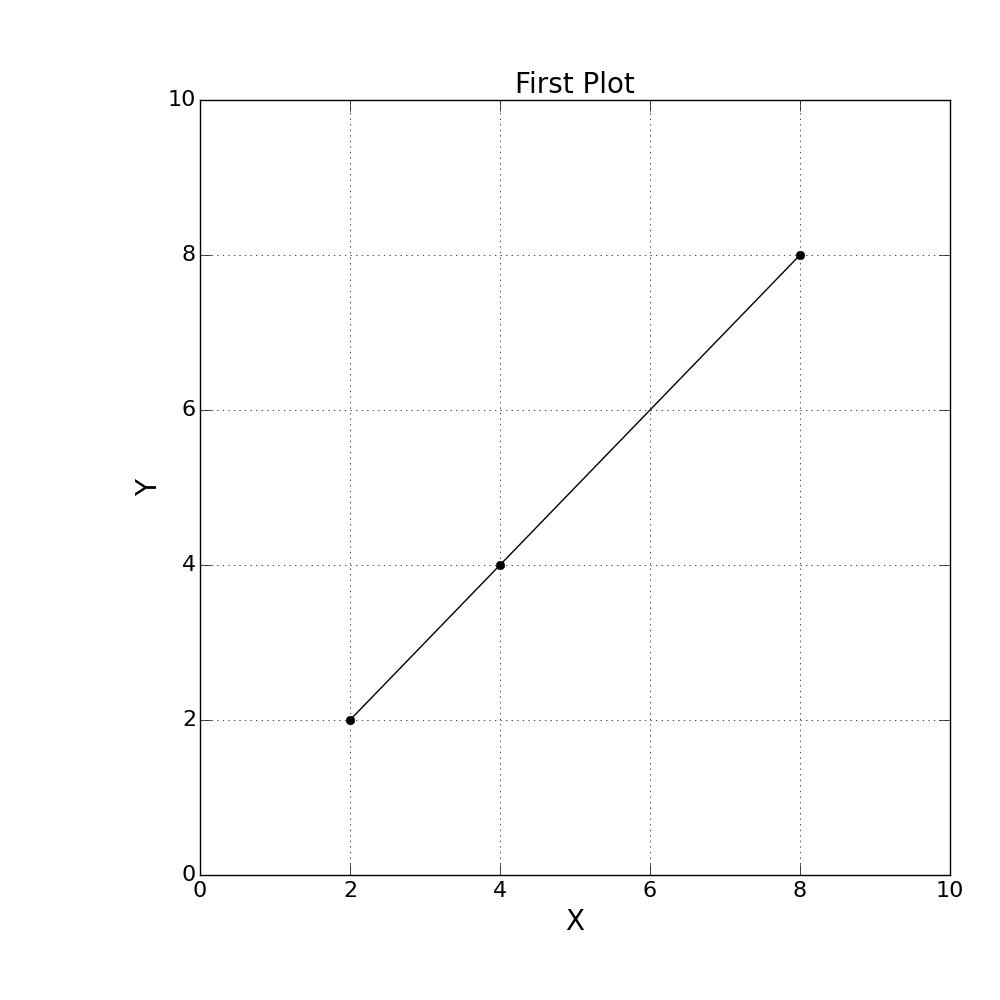
\includegraphics[width=1\linewidth]{../Python/LinePlot/lp.png}
      \caption{\it \small{bar}}
        \label{fig:na10}
  \end{subfigure}
  \caption{\it \small{These figures were generated using...}}
    \label{fig:na04-10}
\end{figure}



\end{document}

